\emph{Author}: Verena Roberts @verenanz \emph{Editor}: Alison Seaman
@alisonseaman

\subsubsection{Summary}

Teachers have a reputation of working in isolation, of keeping their
learning to themselves and on their own islands. They are also known for
generously sharing resources with one another. It is this latter trait
that is becoming increasingly important as the role of the educator
continues to expand. As educational technology research specialist
Stephen Downes
\href{http://www.huffingtonpost.com/stephen-downes/the-role-of-the-educator\_b\_790937.html}{observes},
the expectations on teachers have grown from ``being expert in the
discipline of teaching and pedagogy\ldots{}{[}to needing to have{]}
up-to-date and relevant knowledge and experience in it. Even a teacher
of basic disciplines such as science, history or mathematics must remain
grounded, as no discipline has remained stable for very long, and all
disciplines require a deeper insight in order to be taught
effectively.'' It is no longer possible for an educator to work alone to
fulfil each of these roles: the solution is to work and learn in
collaboration with others. This is where peer-based sharing and learning
online, connected/networked learning, or peeragogy, can play an
important role in helping educators.

\subsection{Becoming a connected/networked learner}

The following steps are set out in `phases' in order to suggest possible
experiences one may encounter when becoming connected. It is
acknowledged that every learner is different and these `phases' only
serve as a guide.

\subsection{Phase 1: Taking the plunge}

To help educators begin to connect, the
\href{http://www.google.com/url?q=https\%3A\%2F\%2Fdl.dropbox.com\%2Fu\%2F38904447\%2Fstarter-kit-final.pdf\&sa=D\&sntz=1\&usg=AFQjCNE9sNo1Lz9-zJ0KH48djXeYVoAF4A}{Connected
Educator's Starter Kit} was created during Connected Educator's Month in
August 2012. In the kit, educators will learn the distinction between
connected `educator' and connecter `learner.' The kit also outlines wide
range of Web 2.0 tools like, Twitter, Facebook, wikis, blogs and social
networking to help support the educator-learner through the phases of
connected learning.

The key to becoming a successful `connected educator-learner' involves
spending the time needed to learn how to learn and share in an open,
connected environment. Each stage, tool and community has a learning
curve and nuances of its own. In order to successfully complete each
phase, connected educator-learners will need to reach out and ask for
support from other learners they encounter. In turn, these new connected
educator-learners will need to reciprocate by sharing learning openly.
Not only will it support others' learning but it helps to foster the
conditions necessary for a healthy online learning community.

\subsection{Phase 2: Lurking}

We all begin as lurkers. A learner can be considered a true `lurker'
after reviewing the starter kit, establishing a digital presence
(through a blog or a wiki) or signing up for Twitter and creating a
basic profile containing a photo. In this phase, lurkers will begin to
\href{http://www.google.com/url?q=http\%3A\%2F\%2Fwww.fractuslearning.com\%2F2012\%2F05\%2F25\%2Ftwitter-follow-education-technology\%2F\&sa=D\&sntz=1\&usg=AFQjCNF8grPMuRwU\_ImW9Jk3ZYrg0m9KgQ}{`follow'
other users on Twitter} and observe
\href{http://www.google.com/url?q=http\%3A\%2F\%2Fcybraryman.com\%2Fchats.html\&sa=D\&sntz=1\&usg=AFQjCNFJASZiwfvPbfOzFbHvAunpXfNC1g}{educational
Twitter `chats'}. Lurkers will also begin to seek out other resources
through
\href{http://theinnovativeeducator.blogspot.ca/2012/04/ten-best-education-blogs.html}{blogs},
\href{http://www.google.com/url?q=http\%3A\%2F\%2Fwww.edsocialmedia.com\%2F2011\%2F02\%2Fthe-advantage-of-facebook-groups-in-education\%2F\&sa=D\&sntz=1\&usg=AFQjCNEvc43Q7GqJqS-2S8GhEJ53Ye-j4Q}{Facebook},
\href{http://www.slideshare.net/cmsdsquires/edmodo-for-teachers-guide}{Edmodo}
and
\href{http://www.emergingedtech.com/2012/02/8-great-linkedin-groups-for-educators/}{LinkedIn}
groups.

\subsection{Phase 3: Entering the fray}

The lurker begins to develop into a connected educator-learner once he
or she makes the decision to enter into a dialogue with another user.
This could take the form of a personal blog post, participation on an
education-related
\href{http://edudemic.com/2012/08/education-blogs/?utm\_medium=twitter\&utm\_source=twitterfeed}{blog}~or
\href{http://educationalwikis.wikispaces.com/Examples+of+educational+wikis}{wiki}~or
a an exchange with another Twitter user. Once this exchange takes place,
relationships may begin to form and the work towards building a Personal
Learning Network (PLN) begins.

One such site where such relationships can be built is
\href{http://www.classroom20.com/}{Classroom 2.0}, which was~founded by
\href{http://www.stevehargadon.com/}{Steve Hargadon.}~Through Classroom
2.0, Steve facilitates a number of free online learning opportunities
including~weekly
\href{http://www.google.com/url?q=http\%3A\%2F\%2Fwww.futureofeducation.com\%2Fnotes\%2FPast\_Interviews\&sa=D\&sntz=1\&usg=AFQjCNHVYOvP-w7NTgKp2Fu2AX4YycnPQQ}{Blackboard
Collaborate}~sessions, conferences, book projects and grassroots
cross-country educational-transformation tours. Classroom 2.0 also
offers a supportive Social Ning---a free, social learning space that
provides online conferences and synchronous and recorded interviews with
inspirational educators---for connected~educator-learners around the
world.

\subsection{Phase 4: Building and shaping your PLN}

Just as not every person one meets becomes a friend, it is important to
remember that not every exchange will lead to a co-learning peeragogy
arrangement. It may be sufficient to follow another who provides useful
content without expecting any reciprocation. It is dependent on each
educator-learner to determine who to pay attention to and what learning
purpose that individual or group will serve. It is also up to the
learner-educator to demonstrate to others that he or she will actively
participate.

There are a number of
\href{http://storify.com/digiphile/how-to-build-a-personal-learning-network-on-twitte}{strategies}
one can use when shaping the PLN to learn.~However, one of the best ways
educators can attract a core of \emph{peeragogues} is by sharing
actively and demonstrating active and open learning for others.

There are a number of sites where a new educator-learner can actively
and openly learn. In addition to personal blogging and wikis, other
professional development opportunities include open, online courses and
weekly synchronous online meetings through video, podcasts or other
forms of media. Examples of these opportunities are:
\href{http://connectedlearning.tv/howard-rheingold-social-media-and-peer-learning-mediated-pedagogy-peeragogy}{Connected
Learning TV},
\href{http://techtalktuesdays.global2.vic.edu.au/}{TechTalkTuesdays},
\href{http://learning2gether.pbworks.com/w/page/32206114/volunteersneeded}{VolunteersNeeded},
\href{http://simplek12.com/webinars}{SimpleK12},
\href{http://k12onlineconference.org/}{K12
Online,}~\href{http://www.learnnowbc.ca/educators/moodlemeets/default.aspx}{CEET},~and~\href{http://edtechtalk.com/taxonomy/term/130}{EdTechTalk}.
Alternatively, courses are offered with
\href{https://p2pu.org/en/schools/school-of-ed-pilot/}{P2PU's} School of
Education or a wide variety of other opportunities collected by
\href{http://www.teachthought.com/}{TeachThought}~and Educator's CPD
online. Peggy George, the co-faciliator of the weekly Classroom 2.0 LIVE
Sessions, created a livebinder package of free
`\href{http://www.google.com/url?q=http\%3A\%2F\%2Fwww.livebinders.com\%2Fplay\%2Fplay\_or\_edit\%3Fid\%3D429095\&sa=D\&sntz=1\&usg=AFQjCNHCIdRn64rPwske2vP7xrpWolb-jA}{PD
On Demand}' connected professional development online options for
peeragogy enthusiasts.

\subsection{Stage 5: Extending the digital PLN and connecting
face-to-face}

Over time, once the connected educator-learner has established a refined
PLN, these peeragogues may choose to shift their learning into physical
learning spaces. Some options available for these educator-learners
would include the new `grassRoots unconferences', which include examples
such as: \href{http://educonphilly.org/}{EduCon},
\href{http://davidwees.com/content/what-edcamp}{EdCamps},
\href{http://thatcamp.org/}{THATcamp}~and~\href{http://connectedcanada.org/}{ConnectedCA}.
These conferences are free or extremely low-cost and focus on learning
from and with others. These `unconferences' are typically publicized
through Twitter, Google Apps, and Facebook. Connecting face-to-face with
other peeragogues can strengthen bonds to learning networks and help to
promote their sustainability.

\subsection{Building personal capacity for Education 2.0}

Given the large number of roles now expected of connected educators,
through peeragogy, K--12 educators can now each distribute the load of
the learning among networks. Although learning to connect takes time and
practice, a support network is a natural accompaniment of
relationship-building and open learning. Numerous online sites and
social platforms exist for K--12 educators to connect and learn together
as peeragogues; though the ways in which connections develop are unique.
It is up to each educator to discover a passion and share it with
others!

\subsection{Postscript}

Sylvia Tolisano, Rodd Lucier and Zoe Branigan-Pipen co-created the
infographic below, which explores experiences individuals may encounter
in the journey to become connected learners. It is not only a helpful
entry point for new learner-educators seeking to become peeragogues, but
it also serves as a wonderful example of peeragogy at work.

\begin{center}
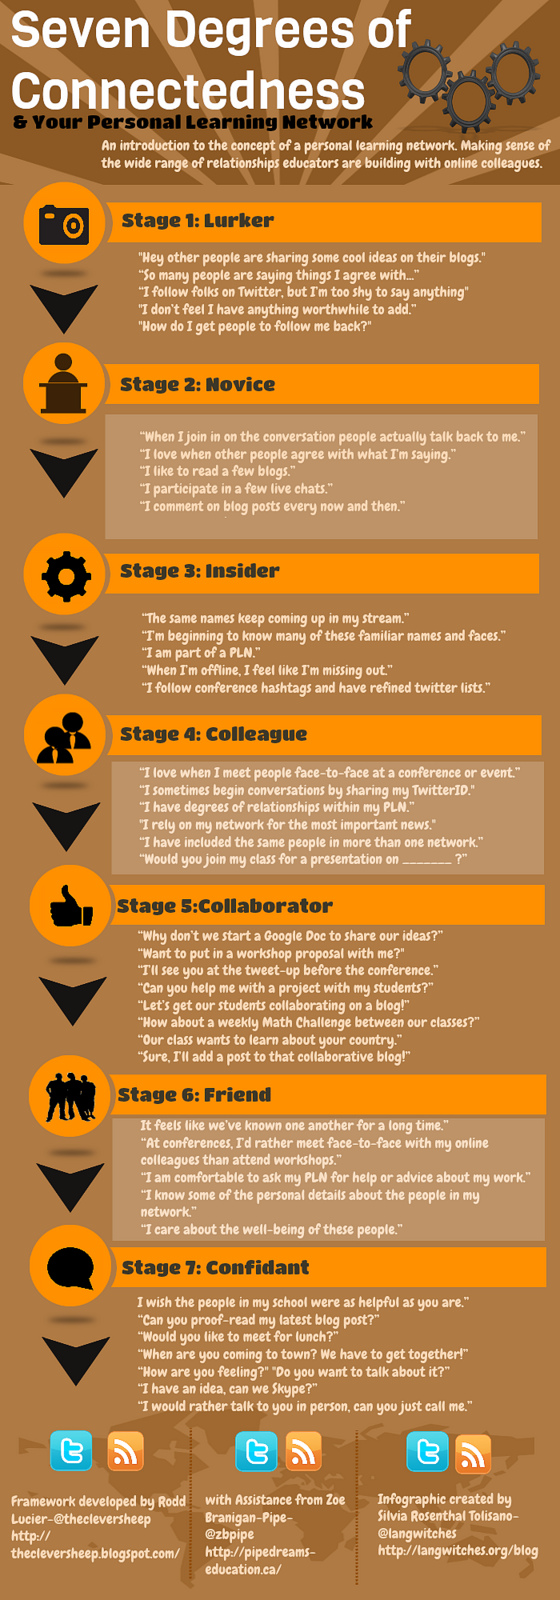
\includegraphics[width=.6\textwidth]{../pictures/k12-infographic.jpg} 
\end{center}

(The image is licensed as CC By-NC-SA, from
\href{http://www.flickr.com/photos/thecleversheep/7161689001/sizes/l/in/photostream/}{Flickr})

Consider taking the plunge into the different stages of a
Networked/Connected Educator today.

\subsection{Additional resources}

\subsubsection{amazing technology tools for your classroom:}

\begin{itemize}
\item
  \href{http://www.freetech4teachers.com/}{Richard Byrne}
\item
  \href{http://langwitches.org/blog/}{Sylvia Tolisano}
\item
  \href{http://catlintucker.com/2011/11/12-tech-tools-that-will-transform-your-classroom/}{Caitlin
  Tucker}
\item
  \href{http://coolcatteacher.blogspot.ca/}{Vicki Davis}
\end{itemize}

\subsubsection{How to develop your PLN:}

\begin{itemize}
\item
  \href{\%20http://thecleversheep.blogspot.ca/2012/06/seven-degrees-of-connectedness\_06.html}{Degrees
  of Connected Teaching} by Rodd Lucier
\item
  \href{\%20http://thecleversheep.blogspot.ca/2012/06/seven-degrees-of-connectedness\_06.html}{TeachThought}
\end{itemize}

\subsubsection{Theory \& philosophy of connnected learning for classroom
transformation:}

\begin{itemize}
\item
  \href{http://pairadimes.davidtruss.com/}{David Truss}
\item
  \href{http://www.downes.ca/presentation/264}{Steven Downes}
\item
  \href{http://willrichardson.com/}{Will Richardson}
\end{itemize}
